
\SGAExposeChapter{X}{Intersecciones en superficies regulares}
\pageoriginale


\begin{center}
\textit{por P. Deligne}
\end{center}

En la primera parte de esta exposición, después de algunos preliminares de teoría de
intersecciones (contenidos en $[5]\cup[7]$), se da la demostración, siguiendo a
Artin, de un caso particular de un teorema de Raynaud [9] (1.13), y una
demostración a priori de un teorema que Néron [8] había verificado caso por caso
(1.15). De (1.13) se deducen con bastante facilidad los teoremas de [9]
utilizados en [2] y, por esta vía, en IX.

En la segunda parte prosigo en la misma línea y explico cómo los ``italianos''
[1], [3] calculaban los números de intersección en las superficies. Los
resultados principales, 2.9 y 2.11, se encuentran asimismo en Northcott [12] y
[13]. Para terminar, doy en 2.27, 2.30 y 2.34 una relación conjetural entre la
dimensión del esquema formal versal de módulos de una singularidad de una curva
reducida, el invariante $\delta$ de la singularidad y un invariante que mide su
simetría.

Esta exposición no se utilizará en lo que sigue del seminario.

\section{Números de intersección en las superficies aritméticas}

\subsection*{1.0}
En este apartado suponemos dados un esquema regular $X$ de dimensión $2$, un
divisor reducido $Y$ de $X$ y un subcuerpo $k$ de
$H^0(Y,\underline{O}_Y)$. Suponemos que $Y$ es una curva (EGA II 7.4.1)
propia sobre $k$. He aquí tres ejemplos de esta situación.

\medskip
\noindent\underline{Ejemplo 1.1.}
Sea $(S,\eta,s)$ un rasgo y sea $f:X\longrightarrow S$ un $S$-esquema
regular, propio y plano sobre $S$, cuyas fibras son puramente de dimensión uno.
Tomamos $Y=(f^{-1}(s))_{\mathrm{red}}$ y $k=k(s)$. A partir de 1.10 nos
restringiremos a este caso.

\pageoriginale

\medskip
\noindent\underline{Ejemplo 1.2.}
Sean $X_o$ el espectro de un anillo local normal de dimensión $2$, $s$ el punto
cerrado de $X_o$ y $f:X\longrightarrow X_o$ un $X_o$-esquema regular y
conexo, propio sobre $X_o$, distinto de $X_o$ pero coincidente con $X_o$ sobre
$X_o\setminus\{s\}$. Tomamos $Y=(f^{-1}(s))_{\mathrm{red}}$ y $k=k(s)$.

\medskip
\noindent\underline{Ejemplo 1.3.}
Tomamos como $X$ una superficie regular completa sobre un cuerpo $k$ y como
$Y$ una curva reducida trazada sobre $X$.

Recordemos el lema siguiente (SGA 6 IV, Ej.~1.9).

\medskip
\noindent\underline{Lema 1.4.}
\underline{Sea} $Z_o$ \underline{un subesquema cerrado de un esquema
noetheriano} $Z$. \underline{Entonces la inclusión de} $Z_o$ \underline{en}
$Z$ \underline{induce un isomorfismo del grupo de Grothendieck de la categoría
de los haces coherentes de} $\underline{O}_{Z_o}$\underline{-módulos sobre el
grupo de Grothendieck de la categoría de los haces coherentes sobre} $Z$
\underline{con soporte en} $Z_o$.

Este lema permite definir la característica de Euler--Poincaré
$\chi(\mathcal F)$ de un haz coherente $\mathcal F$ sobre $X$ con soporte en
$Y$, de manera que:

\medskip
\noindent (i) Si $\mathcal F$ es un haz coherente de
$\underline{O}_Y$-módulos, entonces
\begin{equation}\tag{1.4.1}
\chi(\mathcal F)=\dim_k H^0(\mathcal F)-\dim_k H^1(\mathcal F).
\end{equation}

\noindent (ii) $\chi$ es aditiva respecto de las sucesiones exactas cortas.

Si los haces de cohomología de un complejo $K$ de
$\underline{O}_X$-módulos son haces coherentes con soporte en $Y$, ponemos
\begin{equation}\tag{1.4.2}
\chi(K)=\sum_i(-1)^i\chi(\underline{H}^i(K)).
\end{equation}
Si $\mathcal F$ está concentrado en un punto $y$ de $Y$, se tiene
\begin{equation}\tag{1.4.3}
\chi(\mathcal F)=\operatorname{long}_{\underline{O}_y}(\mathcal F_y)
[k(y):k].
\end{equation}

\pageoriginale

Bajo las hipótesis de (1.1), (1.2) o (1.3), se tiene
\begin{equation}\tag{1.4.4}
\chi(\mathcal F)=\operatorname{long} f_*\mathcal F-
\operatorname{long} R^1f_*\mathcal F.
\end{equation}
Sean $D$ un divisor $\geq0$ con soporte en $Y$ y $\mathcal L$ un haz
invertible sobre $D$. Hay entonces una única manera de definir el grado
$\deg_D(\mathcal L)$ de modo que
\begin{equation}\tag{1.4.5}
\left\{
\begin{array}{l}
\deg_D(\mathcal L'\otimes\mathcal L'')=
\deg_D(\mathcal L')+\deg_D(\mathcal L''),\\[3ex]
\text{para }\mathcal L\subset\underline O,
\text{ se tiene }\deg_D(\mathcal L)=-\chi(\underline O/\mathcal L).
\end{array}
\right.
\end{equation}
Se tiene entonces la fórmula de Riemann--Roch sobre $D$:
\begin{equation}\tag{1.4.6}
\chi(\mathcal L)=\chi(\underline{O}_D)+\deg_D(\mathcal L).
\end{equation}
Sea $D=\sum n_iD_i$ la descomposición de $D$ en divisores irreducibles
reducidos; se tiene
\begin{equation}\tag{1.4.7}
\deg_D(\mathcal L)=\sum n_i\deg_{D_i}(\mathcal L).
\end{equation}

\medskip
\noindent\underline{Definición 1.5.}
\underline{Sean} $D$ \underline{y} $E$ \underline{dos divisores} $\geq0$
\underline{sobre} $X$, \underline{y supongamos que} $D$ \underline{tiene
soporte en} $Y$. \underline{Se define el número de intersección de} $D$
\underline{y} $E$ \underline{(respecto del cuerpo} $k$ (1.0)) \underline{por}
\begin{equation*}
(D,E)=\chi(\underline{O}_D\overset{\mathbb L}{\otimes}\underline{O}_E)
=\chi(\underline{O}_D\otimes\underline{O}_E)
-\chi(\operatorname{Tor}^1(\underline{O}_D,\underline{O}_E)).
\end{equation*}
En efecto, bajo las hipótesis formuladas se tiene
$\operatorname{Tor}^2(\underline{O}_D,\underline{O}_E)=0$.

\medskip
\noindent\underline{Proposición 1.6.}
\underline{Bajo las hipótesis de} 1.5, \underline{se tiene}:

\medskip
\noindent (i) \quad \underline{El número de intersección} $(D,E)$
\underline{es aditivo en los divisores} $D$ \underline{y} $E$;
\underline{esto permite definir por linealidad el número de intersección de dos
divisores no necesariamente positivos.}

\pageoriginale

\noindent (ii) \quad $(D,E)=\deg_D(\underline O(E))$.

\noindent (iii) \quad \underline{Si} $D$ \underline{y} $E$
\underline{solo se cortan en un número finito de puntos, entonces}
$(D,E)=\chi(\underline{O}_D\otimes\underline{O}_E)\geq0$,
\underline{y la igualdad solo puede darse si} $D$ \underline{y} $E$
\underline{son disjuntos.}

\noindent (iv) \quad \underline{Si} $D$ \underline{y} $E$
\underline{tienen soporte en} $Y$, \underline{entonces} $(D,E)=(E,D)$.

\noindent (v) \quad \underline{Si} $N$ \underline{es el haz conormal de}
$D$, \underline{entonces}
\begin{equation*}
D^2=(D,D)=-\deg_D(N).
\end{equation*}

\noindent (vi) \quad \underline{Si} $E$, \underline{no necesariamente
positivo, es el divisor de una función meromorfa sobre} $X$,
\underline{entonces} $(D,E)=0$.

\medskip
\noindent\underline{Demostración.}
La sucesión exacta
\begin{equation*}
0\longrightarrow\underline O(-E)\longrightarrow\underline O_X
\longrightarrow\underline O_E\longrightarrow0
\end{equation*}
da, por (1.4.6),
\begin{equation*}
\begin{array}{rl}
(D,E)\overset{\mathrm{def}}{=}&
\chi(\underline{O}_D\overset{\mathbb L}{\otimes}\underline{O}_E)\\
=&\chi(\underline{O}_D\overset{\mathbb L}{\otimes}\underline{O}_X)
-\chi(\underline{O}_D\overset{\mathbb L}{\otimes}\underline O(-E))\\[1ex]
=&\chi(\underline{O}_D)-\chi(\underline O(-E)|D)
=-\deg_D(\underline O(-E))=\deg_D(\underline O(E)).
\end{array}
\end{equation*}
Esto demuestra (ii), (vi) y la biaditividad, en virtud de (1.4.5) y (1.4.7).
Bajo las hipótesis de (iii), se tiene
$\operatorname{Tor}^1(\underline{O}_D,\underline{O}_E)=0$, de donde se sigue
la conclusión. Bajo las hipótesis de (v), se tiene
\begin{equation*}
\underline{O}_D\otimes\underline{O}_D=\underline{O}_D
\quad\text{y}\quad
\operatorname{Tor}^1(\underline{O}_D,\underline{O}_D)\simeq N
\quad(\text{SGA 6 VII 2.5}),
\end{equation*}
de donde
\begin{equation*}
(D,D)=\chi(\underline{O}_D)-\chi(N)=-\deg_D(N).
\end{equation*}
Por último, (iv) resulta de la simetría del producto tensorial.

Obsérvese que (ii), (iv) y (vi) siguen siendo verdaderos sin suponer positivos
los divisores.

\pageoriginale

\medskip
\noindent\underline{Proposición 1.7.}
\underline{Sean} $(Y_i)_{1\leq i\leq k}$ \underline{las componentes
irreducibles de} $Y$, $f$ \underline{una función meromorfa sobre} $X$,
\underline{y}
\begin{equation*}
\operatorname{div}(f)=\sum_i n_iY_i+Z
\end{equation*}
\underline{su divisor, con} $|Z|\cap Y$ \underline{finito. Entonces, poniendo}
$D_i=n_iY_i$, \underline{se tiene, para} $(a_i)\in\mathbb Q^k$:
\begin{equation*}
\left(\sum_i a_iD_i\right)^2
=-\sum_{i<j}(a_i-a_j)^2(D_i,D_j)-\sum_i a_i^2(D_i,Z).
\end{equation*}

\medskip
\noindent\underline{Demostración} (siguiendo [7]).
En virtud de 1.6 (v), (vi),
\begin{equation*}
\begin{aligned}
\left(\sum_i a_iD_i\right)^2
&=\sum_i a_i\left(D_i,\sum_j a_jD_j\right)
=\sum_i a_i\left(D_i,\sum_j a_jD_j-a_i\operatorname{div}f\right)\\
&=\sum_i a_i\left(D_i,\sum_{j\ne i}(a_j-a_i)D_j-a_iZ\right)\\
&=\sum_{i\ne j}a_i(a_j-a_i)(D_i,D_j)-\sum_i a_i^2(D_i,Z)\\
&=-\sum_{i<j}(a_i-a_j)^2(D_i,D_j)-\sum_i a_i^2(D_i,Z).
\end{aligned}
\end{equation*}

\medskip
\noindent\underline{Corolario 1.8.}
\underline{Bajo las hipótesis del Ejemplo} 1.1, \underline{tomemos como} $f$
\underline{un uniformizante} $\pi$ \underline{de} $S$. \underline{Aquí}
$Z=0$ \underline{y}
\begin{equation*}
\left(\sum_i k_iY_i\right)^2
=-\sum_{i<j}\frac{1}{n_in_j}(k_in_j-k_jn_i)^2(Y_i,Y_j);
\end{equation*}
\underline{por tanto, la forma de intersección es negativa y, si} $Y$
\underline{es conexo, su núcleo está formado precisamente por los múltiplos de}
$\operatorname{div}(\pi)$.

\medskip
\noindent\underline{Corolario 1.9} (Mumford [7]).
\underline{Bajo las hipótesis del Ejemplo} 1.2, \underline{tomemos como} $f$
\underline{un elemento no nulo del ideal maximal del anillo local}
$\underline O_{\sisi{a}{s}}$. \underline{Aquí} $Z>0$, \underline{de modo que la forma de
intersección es definida negativa}.

\pageoriginale

\subsection*{1.10}
\underline{En lo que sigue nos restringimos al caso considerado en el Ejemplo}
1.1.

Lichtenbaum [5] demostró que, en este caso, $X$ es automáticamente proyectivo
sobre $S$, de modo que no hay dificultad en definir el complejo
$Rf^{!}\underline{O}_S$ ([4] III 8.7, p.~190). Puesto que $f$ es de dimensión
relativa $1$ y que $X$ y $S$ son regulares (bastaría que fueran de Gorenstein),
existe ([4] V 8.3 y V 9.1) un haz invertible $\omega_{X/S}$ sobre
$\sisi{S}{X}$, único salvo isomorfismo único, tal que
\begin{equation}\tag{1.10.1}
Rf^{!}\underline{O}_S\simeq\omega_{X/S}[1].
\end{equation}
Designamos por $K$ un divisor cualquiera (efectivo o no) tal que
$\omega_{X/S}\simeq\underline{O}(K)$.

Sea $D$ un divisor $\geq0$ con soporte en $Y$, y sea $N$ su haz conormal:
\begin{center}
\begin{tikzcd}[column sep=large, row sep=large]
D \arrow[rr, "i"] \arrow[dr, swap, "g"] & {} & X \arrow[dl, "f"] \\
{} & S & {}
\end{tikzcd}
\end{center}
Se tiene
\begin{equation}\tag{1.10.2}
Rg^{!}\underline{O}_S
=Ri^{!}Rf^{!}\underline{O}_S
=Ri^{!}\omega_{X/S}[1]
=\omega_{X/S}\big|_D\otimes N^{\vee}[0].
\end{equation}
En virtud del teorema de dualidad ([4] V 11.1, p.~210),
\begin{equation}\tag{1.10.3}
Rg_*Rg^{!}\underline{O}_S
\simeq\operatorname{RHom}(Rg_*\underline{O}_D,\underline{O}_S).
\end{equation}
Además, para todo $\underline{O}_S$-módulo $M$ concentrado en el punto cerrado,
se tiene
\begin{equation}\tag{1.10.4}
\chi\bigl(\operatorname{RHom}(M,\underline{O}_S)\bigr)=-\chi(M),
\end{equation}
de modo que aquí, usando (1.4.4) y (1.10.3), obtenemos
\begin{equation*}
\chi(Rg^{!}\underline{O}_S)=-\chi(\underline{O}_D).
\end{equation*}
Como, por (1.4.6),
\begin{equation*}
\chi(Rg^{!}\underline{O}_S)
=\chi(\underline{O}_D)+\deg_D(Rg^{!}\underline{O}_S),
\end{equation*}

\pageoriginale

deducimos de (1.10.2) que
\begin{equation*}
-2\chi(\underline{O}_D)
=\deg_D(Rg^{!}\underline{O}_{\sisi{D}{S}})
=\deg_D(\omega_{X/S}|_D\otimes N^{\vee})
=\deg_D(\omega_{X/S})-\deg_D(N),
\end{equation*}
lo cual, por 1.6\sisi{}{ }(ii) y (v), puede reformularse del modo siguiente.

\medskip
\noindent\underline{Proposición 1.11.}
\underline{Bajo las hipótesis de} (1.1), \underline{para todo divisor}
$D\geq0$ \underline{con soporte en} $Y$, \underline{se tiene}
\begin{equation*}
\chi(\underline{O}_D)=-\frac12(D,D+K).
\end{equation*}

\subsection*{1.12}
Designamos por $d$ el máximo común divisor de las multiplicidades geométricas de
las componentes irreducibles de $X_s=f^{-1}(s)$; es decir, el máximo común
divisor de las longitudes de los anillos locales en los puntos genéricos de la
fibra especial geométrica de $f$. Si $X_\eta$ tiene un punto racional, o de
manera equivalente si $f:X\longrightarrow S$ tiene una sección $x$, entonces
$d=1$; más precisamente, $f$ es liso en $x(s)$. En efecto, $x$ es una inmersión
cerrada de esquemas regulares, por tanto una inmersión regular, y se aplica EGA
IV 17.12.1.

He aquí la demostración de Artin de un caso particular de un teorema de Raynaud
[9], en la que solo se supone que $d$ es primo con la característica $p$ de
$k$.

\medskip
\noindent\underline{Teorema 1.13.}
\underline{Con la notación precedente, si} $Y$ \underline{es geométricamente
conexo y} $d=1$, \underline{entonces} $X$ \underline{es cohomológicamente
plano sobre} $S$ \underline{en dimensión} $0$ (EGA III 7.8.1);
\underline{más precisamente} (EGA III 7.6.9(ii)), \underline{se tiene}
\begin{equation*}
k\xrightarrow{\;\sim\;}H^0(X_s,\underline{O}_{X_s}).
\end{equation*}
Es fácil reducirse al caso en que $S$ es estrictamente local. Puesto que $Y$ es
geométricamente conexo, $H^0(Y,\underline{O}_Y)$ es una extensión puramente
inseparable de $k$; y puesto que $(d,p)=1$, al menos una componente irreducible
de $Y$ es

\pageoriginale

geométricamente reducida. Se deduce fácilmente que
$H^0(Y,\underline{O}_Y)=k$.

Sea $D$ un divisor sobre $X$ tal que
\begin{equation*}
Y\leq D<X_s.
\end{equation*}
Como $d=1$, $D$ no es un múltiplo racional de $X_s$; por tanto, por 1.8,
\begin{equation*}
(D,X_s-D)=-(D,D)>0.
\end{equation*}
El divisor $Y$ tiene, pues, una componente irreducible $E$ tal que
\begin{equation*}
0<E\leq X_s-D\quad\text{y}\quad(D,E)>0.
\end{equation*}
Consideremos el diagrama
\begin{center}
\begin{tikzcd}[column sep=large, row sep=large]
0 \arrow[r] & \underline{O}(-D-E) \arrow[r] \arrow[d, "\varphi"] &
\underline{O} \arrow[r] \arrow[d, equal] &
\underline{O}_{D+E} \arrow[r] \arrow[d, "\psi"] & 0 \\
0 \arrow[r] & \underline{O}(-D) \arrow[r] &
\underline{O} \arrow[r] & \underline{O}_D \arrow[r] & 0
\end{tikzcd}
\end{center}
El lema de la serpiente da un isomorfismo entre $\operatorname{Ker}(\psi)$ y
$\operatorname{Coker}(\varphi)$. Este conúcleo es precisamente la restricción
de $\underline{O}(-D)$ a $E$, de donde resulta una sucesión exacta
\begin{equation*}
0\longrightarrow\underline{O}(-D)|_E
\longrightarrow\underline{O}_{D+E}
\longrightarrow\underline{O}_D\longrightarrow0.
\end{equation*}
Por construcción,
\begin{equation*}
\sisi{\deg_E(\underline{O}(-D)}{\deg_E(\underline{O}(-D)|_E}=-(D,E)<0,
\end{equation*}
de modo que $H^0(\underline{O}(-D)|_E)=0$ y la aplicación de restricción
\begin{equation*}
0\longrightarrow H^0(\underline{O}_{D+E})
\longrightarrow H^0(\underline{O}_D)
\end{equation*}
es inyectiva. Esto permite construir por inducción una sucesión de divisores
\begin{equation*}
Y=D_0\leq D_1\leq\cdots\leq D_n=X_s
\end{equation*}
tal que $H^0(\underline{O}_{D_i})$ se inyecta en
$H^0(\underline{O}_{D_{i-1}})$. Por consiguiente,
$H^0(\underline{O}_{X_s})=H^0(\underline{O}_Y)=k$, lo que termina la
demostración de 1.13.

\pageoriginale

El hecho siguiente se demuestra en [5] o [10].

\medskip
\noindent\underline{Teorema 1.14} (Castelnuovo, Enriques, \ldots).
\underline{Bajo las hipótesis de} (1.1), \underline{sea} $D$ \underline{un
divisor irreducible reducido contenido en} $Y$. \underline{Supongamos que}
$H^1(D,\underline{O}_D)=0$ \underline{y que, poniendo}
$k'=H^0(D,\underline{O}_D)$, \underline{se tiene}
\begin{equation*}
(D,D)=-[k':k].
\end{equation*}
\underline{Entonces} $D$ \underline{es una recta proyectiva sobre} $k'$,
\underline{y existen un} $S$\underline{-esquema regular} $X_1$,
\underline{un punto cerrado} $x_1$ \underline{de} $X_1$ \underline{con cuerpo
residual} $k'$, \underline{y un isomorfismo de} $X$ \underline{sobre el}
$S$\underline{-esquema obtenido de} $X_1$ \underline{por explosión de} $x_1$,
\underline{bajo el cual} $D$ \underline{se identifica con la fibra sobre}
$x_1$.

Un divisor $D$ que posee estas propiedades se denomina una
\underline{curva excepcional de primera especie}.

No puedo resistir el placer de demostrar la proposición siguiente de Néron [8],
Proposición 1$'$, p.~90.

\medskip
\noindent\underline{Proposición 1.15.}
\underline{Supongamos que} $X_\eta$ \underline{es una curva elíptica (en
particular, que tiene una sección), y que} $X$ \underline{no contiene ninguna
curva excepcional de primera especie. Entonces, con la notación de} (1.10.1),
\underline{la aplicación canónica}
\begin{equation*}
f^*f_*\omega_{X/S}\xrightarrow{\;\sim\;}\omega_{X/S}
\end{equation*}
\underline{es un isomorfismo después de todo cambio de base}.

Como $d=1$ (1.12), por (1.13) basta demostrar que $\omega_{X/S}$ es isomorfo a
$\underline{O}_X$. Puesto que $\omega_{X/S}$ es trivial sobre la curva elíptica
$X_\eta$, sabemos a priori que
\begin{equation*}
\omega_{X/S}\simeq\underline{O}\Bigl(\sum_i n_iY_i\Bigr),
\end{equation*}

\pageoriginale

donde los $Y_i$ son las componentes irreducibles de $Y$; y, puesto que
$\operatorname{div}(\pi)\sim0$, podemos suponer positivos los $n_i$. Si
$\sum_i n_iY_i$ es proporcional a $\operatorname{div}(\pi)$, es un múltiplo
entero de $\operatorname{div}(\pi)$ y hemos terminado. En caso contrario,
\begin{equation*}
\Bigl(\sum_i n_iY_i\Bigr)^2<0,
\end{equation*}
existe un $i$ tal que
\begin{equation*}
\Bigl(Y_i,\sum_j n_jY_j\Bigr)<0,
\end{equation*}
y se aplica el lema siguiente.

\medskip
\noindent\underline{Lema 1.16.}
\underline{Bajo las hipótesis de} 1.1, \underline{supongamos que} $Y$
\underline{es conexo y que, o bien} $Y$ \underline{es reducible, o bien}
$\chi(\underline{O}_Y)\leq0$. \underline{Entonces una componente irreducible}
$Y_i$ \underline{de} $Y$ \underline{es una curva excepcional de primera especie
si y solo si} $(Y_i,K)<0$.

Sea $k'=H^0(Y_i,\underline{O}_{Y_i})$. La fórmula de Riemann--Roch 1.11 da
\begin{equation*}
\chi(\underline{O}_{Y_i})
=[k':k]\bigl(1-\dim_{k'}H^1(Y_i,\underline{O}_{Y_i})\bigr)
=-\frac12\bigl((Y_i,Y_i)+(Y_i,K)\bigr).
\end{equation*}
Si $Y_i$ es excepcional de primera especie, se sigue que
$(Y_i,K)=-[k':k]<0$. Recíprocamente, si $(Y_i,K)<0$, entonces
$\chi(\underline{O}_{Y_i})>0$, lo que implica
$\chi(\underline{O}_{Y_i})=[k':k]$ y que $Y$ es reducible. Por tanto, por 1.8,
$(Y_i,Y_i)<0$. Los enteros negativos $(Y_i,Y_i)$ y $(Y_i,K)$ son divisibles por
$[k':k]$ y, por consiguiente, necesariamente
\begin{equation*}
(Y_i,Y_i)=(Y_i,K)=-[k':k].
\end{equation*}

\medskip
\noindent\underline{Ejercicio.}
(a) Bajo las hipótesis de (1.1), supongamos que $X_\eta$ es un espacio homogéneo
principal bajo una curva elíptica y que $X$ no contiene ninguna curva
excepcional de primera especie. Demostrar que sobre $X$ la fórmula de
Riemann--Roch (1.11) toma la forma
\begin{equation*}
\chi(\underline{O}_D)=-\frac12(D,D).
\end{equation*}

\pageoriginale

(b) Supongamos además que el cuerpo residual $k(s)$ es algebraicamente cerrado.
Demostrar que el diagrama de las componentes irreducibles de $X_s$ es un
múltiplo de uno de los diagramas considerados por Néron [8], pp.~124--125,
cuarta columna (casos del a al c8). El diagrama determina los géneros de las
componentes irreducibles reducidas, sus multiplicidades en $X_s$ y la naturaleza
y disposición de las singularidades de $(X_s)_{\mathrm{red}}$.

Trátese primero el caso en que $X_s$ es irreducible. Una vez excluido este caso,
demuéstrese que toda componente irreducible reducida es una recta proyectiva de
autointersección $-2$. Si $X_s=\sum_i n_iD_i$ es la descomposición de $X_s$ en
divisores irreducibles reducidos, reescríbase esta condición como
\begin{equation}\tag{*}
n_i=\frac12\sum_{j\ne i}\sisi{n_i}{n_j}(D_i,D_j).
\end{equation}
Por otra parte, $X_s$ es conexo, de modo que:

\medskip
\noindent (**) Para cualesquiera $i$ y $j$, existe una cadena
$i=i_1,i_2,\ldots,i_n=j$ tal que
$(D_{i_k},D_{i_{k+1}})\ne0$.

Hállense ahora todas las soluciones enteras de $(*)+(**)$. Demuéstrese primero
que, salvo en los casos b2 y c2 de Néron, los números de intersección
$(D_i,D_j)$ son cero o uno.

\section{Intersecciones a la italiana}

Sean $S'$ y $S$ dos superficies proyectivas lisas sobre un cuerpo $k$, y sea
$f:S'\longrightarrow S$ un morfismo birracional. Si $D$ y $E$ son dos
divisores sobre $S$, entonces
\begin{equation*}
(D,E)=(f^*D,f^*E),
\end{equation*}

\pageoriginale

como se ve, por ejemplo, desplazando $D$ y $E$.

Es natural, por tanto, buscar una expresión ``birracional'' para el número de
intersección. Me propongo explicar cómo procedían los italianos. Mi fuente
principal de información es [1], que contiene una extensa bibliografía. Véanse
también Manin [6] y Northcott [12], [13].

\subsection*{2.0}
Sea $S$ el espectro de un anillo local regular de dimensión $2$, sea $s$ el
punto cerrado de $S$ y sea $k$ un subcuerpo de $k(s)$ tal que $k(s)$ sea finito
sobre $k$. Los números de intersección y las características de
Euler--Poincaré se calcularán sobre $k$.

En esta sección, un $S$-esquema $p:S'\longrightarrow S$ se denominará una
\underline{transformación birracional de} $S$ si es regular y conexo, y si $p$
es propio e induce un isomorfismo
$S'\setminus p^{-1}(s)\longrightarrow S\setminus\{s\}$. Todo lo que se diga
sobre $S$ será igualmente aplicable a las localizaciones de sus transformaciones
birracionales en un punto cerrado.

\subsection*{2.1}
Sea $f:(S'',p'')\longrightarrow(S',p')$ un morfismo de $S$-esquemas entre
transformaciones birracionales de $S$. Se sabe [5] que $f$ tiene una
factorización única
\begin{equation*}
f=f_n\cdots f_1,\qquad f_i:S_{i+1}\longrightarrow S_i,
\end{equation*}
tal que $S_{i+1}$ se obtiene de $S_i$ por explosión de un conjunto finito $X_i$
de puntos cerrados, y $f_i(X_{i+1})\subset X_i$. El conjunto $X_i$ es el
conjunto de puntos de $S_i$ en los que la proyección de $S''$ sobre $S_i$ no es
un isomorfismo.

En particular, $f$ induce un isomorfismo sobre el complementario de un
subconjunto finito de $S'$ que contiene los puntos genéricos de las componentes
irreducibles de $p'^{-1}(s)$. Por consiguiente, $f^{-1}$ define una inyección

\pageoriginale

del conjunto $\operatorname{Irr}(p'^{-1}(s))$ de las componentes irreducibles de
$p'^{-1}(s)$ en $\operatorname{Irr}(p''^{-1}(s))$.

Las transformaciones birracionales de $S$ no tienen automorfismos sobre $S$.
Designamos por $I$ el conjunto de las clases de $S$-isomorfía de transformaciones
birracionales de $S$, ordenado por dominación. El conjunto $I$ es filtrante por
la derecha y tiene elemento mínimo $S$.

\medskip
\noindent\underline{Definición 2.2.}
\underline{El conjunto} $S^*$ \underline{de los puntos de} $S$
\underline{infinitamente próximos a} $s$ \underline{es el conjunto límite
inductivo}
\begin{equation*}
S^*=\varinjlim_I\operatorname{Irr}(p^{-1}(s)).
\end{equation*}
Si un elemento $t\in S^*$ está representado sobre una transformación
birracional $S'$ de $S$ por una curva completa irreducible reducida $T$, el
cuerpo $H^0(T,\underline{O}_T)$ depende únicamente de $t$, y no de la elección
de $S'$. Se denomina el \underline{cuerpo residual} $k(t)$ de $t$.

Sea $S_1$ la explosión de $S$ a lo largo de $s$. La recta proyectiva $s^*$,
imagen inversa de $\{s\}$ en $S_1$, se denomina la \underline{curveta} de $s$ y
define un elemento $s^*$ de $S^*$ con cuerpo residual $k(s)$.

Sea $S'$ una transformación birracional de $S$, sea $t$ un punto cerrado de
$S'$ y sea $S'_t$ el espectro del anillo local de $S'$ en $t$. Hay una inyección
evidente $(S'_t)^*\hookrightarrow S^*$; en particular, $t$ define un elemento
$t^*$ de $S^*$ con el mismo cuerpo residual. Designamos por $(S')^*$ la unión,
en $S^*$, de los $(S'_t)^*$, cuando $t$ recorre los puntos cerrados de $S'$.

La proposición siguiente se deduce de la descripción 2.1 de las transformaciones
birracionales de $S$.

\pageoriginale

\medskip
\noindent\underline{Proposición 2.3.}
\underline{Para todo} $t\in S^*$, \underline{existe una única sucesión de
transformaciones birracionales} $(S_i)_{0\leq i\leq n+1}$ \underline{de} $S$
\underline{y de puntos cerrados} $t_i\in S_i$ $(0\leq i\leq n)$
\underline{tales que}:

\medskip
\noindent (i)\quad $S_0=S$, \underline{y} $S_{i+1}$ \underline{es la explosión
de} $S_i$ \underline{a lo largo de} $\{t_i\}$;

\noindent (ii)\quad $t_{i+1}\in t_i^*$ $(0\leq i<n)$, \underline{y}
$t=t_n^*$.

\medskip
\noindent\underline{Además, para toda transformación birracional} $(S',p')$
\underline{de} $S$, \underline{el elemento} $t$ \underline{pertenece a la
imagen de} $\operatorname{Irr}(p'^{-1}(s))$ \underline{en} $S^*$
\underline{si y solo si} $S'$ \underline{domina} $S_{n+1}$.

El entero $n$ se denomina el orden de $t$. Designamos por $S(t)$
(respectivamente, $S_+(t)$) la transformación birracional $S_n$
(respectivamente, $S_{n+1}$) de $S$. Por abuso de notación, designamos también
por $t$ el punto cerrado $t_n$ de $S_n$, y por $t^*$ su imagen inversa $t_n^*$
en $S_{n+1}$.

Dotamos a $S^*$ del orden siguiente:
\begin{equation*}
t_1\prec t_2
\quad\Longleftrightarrow\quad
S_+(t_2)\ \text{domina}\ S_+(t_1).
\end{equation*}
Si $t_1\prec t_2$, entonces $k(t_2)$ es una extensión de $k(t_1)$. El conjunto
ordenado $S^*$ tiene elemento mínimo $s^*$, y todo subconjunto acotado de $S^*$
es finito y totalmente ordenado ($S^*$ es un ``árbol con raíz $s^*$''). Además,
el orden $n$ de $t\in S^*$ es la distancia, en el árbol $S^*$, de $s^*$ a $t$.

La proposición siguiente hace explícita la descripción 2.1 de las
transformaciones birracionales de $S$.

\medskip
\noindent\underline{Proposición 2.4.}
\underline{La función que asigna a una transformación birracional}
$p:S'\to S$ \underline{el subconjunto} $\operatorname{Irr}(p^{-1}(s))$
\underline{de} $S^*$ \underline{induce una biyección entre} $I$ (2.1)
\underline{y los subconjuntos finitos de} $S^*$ \underline{que, junto con cada
elemento,}

\pageoriginale

\underline{contienen todos sus predecesores}.

Sea $D$ un divisor $\geq0$ sobre $S$, y sea $t\in S^*$. Se dice que $t$
\underline{pertenece a} $D$ si el punto cerrado $t$ de $S(t)$ (2.3) pertenece a
la transformada estricta (la adherencia esquemática de $D-\{s\}$) de $D$ sobre
$S(t)$.

\medskip
\noindent\underline{Definición 2.5.}
\underline{Sean} $t,t'\in S^*$. \underline{Se dice que} $t'$ \underline{es
próximo a} $t$ \underline{si} $t'\in S_+(t)^*$ (2.2) \underline{y pertenece a
la curveta} $t^*$ \underline{de} $t$ (2.3).

Si $t'$ es un sucesor inmediato de $t$, entonces $t'$ es próximo a $t$. Si, en
una sucesión $(t_i)_{0\leq i\leq n}$, cada $t_{i+1}$ es un sucesor inmediato de
$t_i$, y si $t_n$ es próximo a $t_0$, entonces todo $t_i$ con $0<i\leq n$ es
próximo a $t_0$, mientras que $t_n$ no es próximo a $t_i$ para
$0<i\leq n-1$.

\subsection*{2.6}
Sea $A$ un anillo local noetheriano de dimensión $n$, sea $T$ su espectro, sea
$m$ su ideal maximal, sea $k=A/m$ su cuerpo residual y sea
$P=\sum_{0\leq i<n}a_iX^i$ su polinomio de Hilbert--Samuel:
\begin{equation*}
P(r)=\dim_k(m^r/m^{r+1})\qquad\text{para }r\text{ suficientemente grande}.
\end{equation*}
Recordemos que la multiplicidad $\mu_s$ del punto cerrado $s$ en $T$ se define
por
\begin{equation*}
a_{n-1}=\frac{\mu_s}{(n-1)!}.
\end{equation*}
Cuando $n=1$, esto dice simplemente
\begin{equation*}
\mu_s=\dim_k(m^r/m^{r+1})\qquad\text{para }r\text{ suficientemente grande}.
\end{equation*}
Geométricamente, $\mu_s$ puede definirse como el grado, en el espacio proyectivo
$\mathbf P_k(m/m^2)$, de la fibra especial de la explosión de $T$ a lo largo del
subesquema cerrado $\{s\}$.

\pageoriginale

Recordemos que, si $Y$ y $Z$ son dos subesquemas cerrados de un esquema $X$,
entonces la transformada estricta de $Y$ en la explosión $\widetilde X$ de $X$
a lo largo de $Z$ ---la adherencia esquemática de $Y\setminus Z$ en
$\widetilde X$--- es precisamente la explosión de $Y$ a lo largo de
$Y\cap Z$.

Supongamos que $T$ es un subesquema cerrado de un esquema regular $U$. Sea
$p:U_1\longrightarrow U$ la explosión de $U$ a lo largo de $\{s\}$, sea $s^*$
la imagen inversa de $s$ en $U_1$ y sea $T'$ la transformada estricta de $T$ en
$U_1$. La discusión precedente muestra que la multiplicidad de $T$ en $s$ es el
grado, en el espacio proyectivo $s^*$, del subesquema $s^*\cap T'$.

Supongamos además que $T$ es un divisor sobre $U$. Sea $T^*$ su transformada
total en $U_1$ (el divisor imagen inversa), y definamos $\nu$ por
$T^*=\nu s^*+T'$. Si $X$ es una recta en $s^*$ y las características de
Euler--Poincaré se calculan como sumas alternadas de dimensiones sobre $k$,
entonces
\begin{equation}\tag{2.6.1}
(X,s^*)=
\chi(\underline{O}_X\overset{\mathbb L}{\otimes}\underline{O}_{s^*})
=\deg_X\underline{O}(s^*)=-1,
\end{equation}
y hemos visto que
\begin{equation}\tag{2.6.2}
(X,T')=
\chi(\underline{O}_X\overset{\mathbb L}{\otimes}\underline{O}_{T'})
=\deg_{s^*}(s^*\cap T')=\mu_s.
\end{equation}
La fórmula de proyección
\begin{equation*}
Rp_*(\underline{O}_X\overset{\mathbb L}{\otimes}\underline{O}_{T^*})
=Rp_*(\underline{O}_X\overset{\mathbb L}{\otimes}Lp^*\underline{O}_T)
=Rp_*\underline{O}_X\overset{\mathbb L}{\otimes}\underline{O}_T
\end{equation*}
y su corolario
\begin{equation*}
(X,T^*)=\nu(X,s^*)+(X,T')=0
\end{equation*}
dan, por (2.6.1) y (2.6.2), la identidad
\begin{equation}\tag{2.6.3}
\mu_s=\nu.
\end{equation}

\pageoriginale

\medskip
\noindent\underline{Proposición 2.7.}
\underline{Sean} $T$ \underline{un divisor} $\geq0$ \underline{sobre un esquema
regular} $U$, $s$ \underline{un punto cerrado de} $U$, $U_1$ \underline{la
explosión de} $U$ \underline{a lo largo de} $\{s\}$, $s^*$ \underline{la
imagen inversa de} $s$ \underline{en} $U_1$, $T'$ \underline{la transformada
estricta de} $T$ \underline{sobre} $U_1$, \underline{y} $T^*$ \underline{su
transformada total}.

\underline{Las tres cantidades siguientes son iguales}:

\medskip
\noindent (i)\quad \underline{la multiplicidad, en el sentido de Samuel, del
punto} $s$ \underline{en} $T$;

\noindent (ii)\quad \underline{el grado, en el espacio proyectivo} $s^*$,
\underline{de} $s^*\cap T'$;

\noindent (iii)\quad \underline{la multiplicidad de} $s^*$ \underline{en el
divisor} $T^*$.

\subsection*{2.8}
Volvamos a las hipótesis de 2.0. Sea $D$ un divisor $\geq0$ sobre $S$ y sea
$t\in S^*$. La \underline{multiplicidad} $\mu_t(D)$ \underline{de} $D$
\underline{en} $t$ es, por definición, la multiplicidad en $t$ de la
transformada estricta de $D$ sobre $S(t)$ (2.3). El soporte de la función
$t\mapsto\mu_t(D)$ es el conjunto de los puntos infinitamente próximos a $s$
que pertenecen a $D$ (2.4). Cuando $D$ es regular, los números
$\mu_t(D)[k(t):k(s)]$ son cero o uno: en efecto, las transformadas estrictas
$D'$ de $D$ son isomorfas a $D$, y se aplica la definición (2.6) de la
multiplicidad.

Los números de intersección pueden calcularse en función de las multiplicidades.

\medskip
\noindent\underline{Teorema 2.9.}
\underline{Si los divisores} $D$ \underline{y} $E$ \underline{solo se cortan
en} $s$, \underline{entonces}
\begin{equation*}
(D,E)=\sum_{t\in S^*}\mu_t(D)\mu_t(E)[k(t):k],
\end{equation*}
\underline{donde la suma se extiende a los puntos infinitamente próximos a}
$s$ \underline{que pertenecen a la vez a} $D$ \underline{y} $E$.

\medskip
\noindent\underline{Demostración.}
Sea $p:S'\longrightarrow S$ una transformación birracional de $S$. Designamos
por $D^*$ y $E^*$ las transformadas totales de $D$ y $E$, y por $D'$ y $E'$ sus
transformadas estrictas.

\pageoriginale

\medskip
\noindent\underline{Lema 2.9.1.}
(i) \underline{La transformada total} $D^*$ \underline{se caracteriza por}:

\medskip
\noindent (a)\quad $D^*-D'$ \underline{tiene soporte en} $p^{-1}(s)$;

\noindent (b)\quad \underline{si} $X$ \underline{tiene soporte en}
$p^{-1}(s)$, \underline{entonces} $(D^*,X)=0$.

\noindent (ii)\quad $(D,E)=(D^*,E^*)=(D^*,E')=(D',E^*)$.

La afirmación (i)(a) es inmediata, y (i)(b) se sigue de 1.6(vi). Que (a) y (b)
determinan $D^*$ se deduce de 1.9. Por construcción, el conúcleo de la
aplicación
\begin{equation*}
\underline{O}_E\longrightarrow
\sisi{f_*\underline{O}_E}{p_*\underline{O}_{E'}}
\end{equation*}
es finito; por tanto,
\begin{equation*}
\begin{aligned}
(D^*,E')
&=\chi(L\sisi{f}{p}^*\underline{O}_D\otimes\underline{O}_{E'})\\
&=\chi(\underline{O}_D\otimes R\sisi{f}{p}_*\underline{O}_{E'})
=\chi(\underline{O}_D\otimes\underline{O}_E)
=(D,E),
\end{aligned}
\end{equation*}
lo que, por (i), implica (ii).

Tomemos como $S'$ la explosión de $S$ en $s$. Por (2.9.1), (2.6.3) y 2.7,
\begin{equation}\tag{2.9.2}
\begin{aligned}
(D,E)
&=(D^*,E')
=\bigl(D'+\mu_s(\sisi{S}{D})s^*,E'\bigr)\\
&=(D',E')+\mu_s(D)(s^*,E')\\
&=(D',E')+\mu_s(D)\mu_s(E)[k(s):k].
\end{aligned}
\end{equation}
El Teorema 2.9 resulta ahora por inducción sobre $(D,E)$, aplicando
repetidamente (2.9.2).

\subsection*{2.10}
Sea $A$ un anillo local noetheriano reducido de dimensión uno, sea $s$ el punto
cerrado de $\operatorname{Spec}(A)$, sea $\widetilde A$ la normalización de $A$ y
sea $k$ un cuerpo sobre el cual $k(s)$ es finito. Supongamos que $\widetilde A$
es finito sobre $A$ (de manera equivalente, que el completado $\widehat A$ es
reducido). El \underline{invariante} $\delta$ \underline{de la singularidad de}
$\operatorname{Spec}(A)$ \underline{en} $s$ es la longitud sobre $k$ del
$A$-módulo $\widetilde A/A$.

\pageoriginale

\medskip
\noindent\underline{Teorema 2.11.}
\underline{Sea} $D$ \underline{una curva reducida sobre} $S$.
\underline{Entonces}:

\medskip
\noindent (i)\quad \underline{para todo} $t\in S^*$, \underline{con la notación
de} 2.8, \underline{se tiene}
\begin{equation*}
\mu_t(D)=
\sum_{\substack{t'\ \text{próximo}\\\text{a }t}}
\mu_{t'}(D)[k(t'):k(t)].
\end{equation*}

\noindent (ii)\quad \underline{Supongamos que la normalización} $\widetilde D$
\underline{de} $D$ \underline{es finita sobre} $D$, \underline{y sea}
$\delta=\chi(\underline{O}_{\widetilde D}/\underline{O}_D)$
\underline{el invariante de la singularidad de} $D$ \underline{en} $s$.
\underline{Para todos salvo un número finito de} $t\in S^*$,
$\mu_t(D)$ \underline{es cero o uno, y}
\begin{equation*}
\delta=\sum_{t\in S^*}\frac12\mu_t(D)
\bigl(\mu_t(D)-1\bigr)[k(t):k].
\end{equation*}

Sea $p:S_1\longrightarrow S$ la explosión de $S$ a lo largo de $\{s\}$, sea
$D^*$ la transformada total de $D$ y sea $D'$ su transformada estricta. Por
(2.7),
\begin{equation}\tag{2.11.1}
D^*=D'+\mu_s(D)s^*
\end{equation}
y
\begin{equation}\tag{2.11.2}
\mu_s(D)=(s^*,D')\,[k(s):k]^{-1}.
\end{equation}
La curveta $s^*$ es no singular. Así, por 2.8 y la Definición 2.5, la fórmula
2.9, aplicada sobre $S_1$ a los divisores $s^*$ y $D'$, se convierte en
\begin{equation}\tag{2.11.3}
(s^*,\sisi{D}{D'})=
\sum_{\substack{t'\ \text{próximo}\\\text{a }s}}
\mu_{t'}(D)[k(t'):k].
\end{equation}
La afirmación (i) para $s=t$ resulta de (2.11.2) y (2.11.3); el caso general se
obtiene aplicando este resultado a la localización de $S(t)$ en $t$ (2.3).

Sea $m$ el ideal maximal que define $\{s\}$ y sea $n\geq0$. Se sabe (SGA VII
3.5) que
\begin{equation}\tag{2.11.4}
p_*\underline{O}_{S_1}(-ns^*)=m^n
\quad\text{y}\quad
R^ip_*\underline{O}_{S_1}(-ns^*)=0\quad(i>0).
\end{equation}

\pageoriginale

De esto y de la sucesión exacta
\begin{equation*}
0\longrightarrow\underline{O}_{S_1}(-ns^*)
\longrightarrow\underline{O}_{S_1}
\longrightarrow\underline{O}_{ns^*}
\longrightarrow0
\end{equation*}
se deduce que
\begin{equation}\tag{2.11.5}
p_*\underline{O}_{ns^*}=\underline{O}_S/m^n
\quad\text{y}\quad
R^ip_*\underline{O}_{ns^*}=0\quad(i>0),
\end{equation}
y que
\begin{equation}\tag{2.11.6}
\chi(\underline{O}_{ns^*})
=\chi(\underline{O}_S/m^n)
=\frac{n(n+1)}2[k(s):k].
\end{equation}
Pongamos $n=0$ en (2.11.4). Para todo complejo $K$ de haces coherentes sobre
$S$, la fórmula de proyección da
\begin{equation*}
K\xrightarrow{\;\sim\;}Rp_*Lp^*K
\qquad
\bigl(\simeq K\overset{\mathbb L}{\otimes}Rp_*\underline{O}_{S_1}\bigr).
\end{equation*}
En particular, como
$L\sisi{f}{p}^*\underline{O}_D=\sisi{f}{p}^*\underline{O}_D=
\underline{O}_{D^*}$, se tiene
\begin{equation}\tag{2.11.7}
\sisi{f}{p}_*\underline{O}_{D^*}=\underline{O}_D
\quad\text{y}\quad
R^i\sisi{f}{p}_*\underline{O}_{D^*}=0\quad(i>0).
\end{equation}
Pongamos $E=\mu_s(D)s^*$. Por (2.11.1), (2.9.1)(i)(b) y (2.6.1),
\begin{equation}\tag{2.11.8}
\begin{aligned}
\chi(\underline{O}_{D'\cap E})
&=(D',E)=(D^*-E,E)=-(E,E)\\
&=-\mu_s(D)^2(s^*,s^*)
=\mu_s(D)^2[k(s):k].
\end{aligned}
\end{equation}
La sucesión exacta
\begin{equation*}
0\longrightarrow\underline{O}_{D^*}
\longrightarrow\underline{O}_{D'}\oplus\underline{O}_E
\longrightarrow\underline{O}_{D'\cap E}
\longrightarrow0
\end{equation*}
da, por imagen directa y (2.11.7), la sucesión exacta
\begin{equation*}
0\longrightarrow\underline{O}_D
\longrightarrow p_*\underline{O}_{D'}\oplus p_*\underline{O}_E
\longrightarrow p_*\underline{O}_{D'\cap E}
\longrightarrow0.
\end{equation*}
Por consiguiente, la rama diplomática conserva la sucesión impresa, mientras
que la rama actual muestra la sucesión cociente exacta:
\ifthenelse{\boolean{original}}{%
\begin{equation*}
0\longrightarrow p_*\underline{O}_{D'}/\underline{O}_D
\longrightarrow p_*\underline{O}_E
\longrightarrow p_*\underline{O}_{D'\cap E}
\longrightarrow0.
\end{equation*}
}{%
\begin{equation*}
0\longrightarrow p_*\underline{O}_E
\longrightarrow p_*\underline{O}_{D'\cap E}
\longrightarrow p_*\underline{O}_{D'}/\underline{O}_D
\longrightarrow0.
\end{equation*}
}

\pageoriginale

Por tanto, por (2.11.6) y (2.11.8),
\begin{equation}\tag{2.11.9}
\begin{aligned}
\chi(p_*\underline{O}_{D'}/\underline{O}_D)
&=\sisi{\frac12\mu_s(D)\bigl(\mu_s(D)+1\bigr)-\mu_s(D)^2}
{\mu_s(D)^2-\frac12\mu_s(D)\bigl(\mu_s(D)+1\bigr)}[k(s):k]\\
&=\frac12\mu_s(D)\bigl(\mu_s(D)-1\bigr)[k(s):k].
\end{aligned}
\end{equation}
Los esquemas $D$ y $D'$ son reducidos, solo difieren sobre $s$, y $D'$ es finito
sobre $D$. Tienen, pues, la misma normalización, y el invariante $\delta$ de la
singularidad de $D$ en $s$ es la suma de
$\chi(p_*\underline{O}_{D'}/\underline{O}_D)$ y de los invariantes $\delta$ de
las singularidades de $D'$ en los puntos de $D'\cap s^*$. Demostramos 2.11(ii)
por inducción sobre $\delta$. Si $\mu_s(D)>1$, se aplica la hipótesis de
inducción a $D'$, y 2.11(ii) se deduce de (2.11.9). Si $\mu_s(D)=1$, entonces
$(D',s^*)=1$ y $D'\cap s^*$ es un divisor regular sobre $D'$; por EGA IV 19.1.1,
$D'$ es regular. La fórmula (2.11.9) muestra entonces que $D$ es regular, y
2.11(ii) se deduce de 2.8.

\subsection*{2.12}
Sea $t\in S^*$, y sea $S'$ una transformación birracional de $S$ que domine
$S_+(t)$ (2.3). La \underline{transformada total} de $t$ sobre $S'$, que
seguimos designando por $t^*$, es la transformada total sobre $S'$ del divisor
$t^*$ sobre $S_+(t)$.

Sea $\nu:S^*\longrightarrow\mathbf N$ una función de soporte finito, y
supongamos que, para todo $t\in S^*$,
\begin{equation}\tag{2.12.1}
\nu(t)\geq
\sum_{\substack{t'\ \text{próximo}\\\text{a }t}}
\nu(t')[k(t'):k(t)]
\end{equation}
(la desigualdad de los puntos próximos). Sea $f:S'\longrightarrow S$ una
transformación birracional de $S$ que domine $S_+(t)$ para todo $t$ del soporte
de $\nu$, y sea
\begin{equation*}
\nu^*=\sum_{t\in S^*}\nu(t)t^*
\end{equation*}
el divisor correspondiente sobre $S'$.

\pageoriginale

Designamos por $I(\nu)$ el ideal de $\underline{O}_S$ obtenido por imagen
directa mediante $f$ del ideal de $\underline{O}_{S'}$ que define $\nu^*$:
\begin{equation*}
I(\nu)=f_*\underline{O}_{S'}(-\nu^*).
\end{equation*}
Por (2.11.4), este ideal no depende de la elección de $S'$. Los ideales de $S$
obtenidos de este modo son los que Zariski [11] denomina ``completos''.

\medskip
\noindent\underline{Teorema 2.13.}
\underline{Bajo las hipótesis precedentes, se tiene}
\begin{equation*}
\chi(\underline{O}_S/I(\nu))
=\sum_{t\in S^*}\frac{\nu(t)(\nu(t)+1)}2[k(t):k],
\end{equation*}
\underline{y}
\begin{equation*}
R^if_*\underline{O}_{S'}(-\nu^*)=0
\quad\text{para }i>0.
\end{equation*}

En francés antiguo, esto se expresa brevemente diciendo: ``imponer a una curva
plana que pase $n$ veces por un punto $t$, propio o infinitamente próximo,
impone $n(n+1)/2$ condiciones, en general independientes, a los coeficientes de
su ecuación''.

Demostremos primero el lema siguiente.

\medskip
\noindent\underline{Lema 2.14.}
\underline{Sea} $p:S_1\longrightarrow S$ \underline{la explosión de} $S$
\underline{a lo largo de} $\{s\}$; \underline{sea} $T$ \underline{un
subesquema cerrado de} $S_1$ \underline{de ideal} $q$;
\sisi{$D$ \underline{un divisor}, }{}\underline{sea} $n$
\underline{un entero}; \underline{sea}
$J=\underline{O}_{S_1}(-s^*)$ \underline{el ideal que define el divisor}
$s^*$; \underline{pongamos}
$Y=\operatorname{Spec}(\underline{O}_{S_1}/J^nq)$; \underline{y sea} $D$
\underline{un divisor regular sobre} $S$, \underline{de transformada estricta}
$D'$ \underline{sobre} $S_1$. \underline{Supongamos que} $T\cap s^*$
\underline{y} $T\cap D'$ \underline{son finitos}.

\medskip
\noindent (i)\quad \underline{Si}
$\operatorname{long}_{k(s)}(T\cap s^*)\leq n+1$, \underline{entonces}
\begin{equation*}
R^ip_*(qJ^n)=0\quad\text{para }i>0,
\end{equation*}
\underline{y, si} $T$ \underline{es artiniano},
\begin{equation*}
\operatorname{long}_{k(s)}
\bigl(\underline{O}_S/p_*(qJ^n)\bigr)
=\frac{n(n+1)}2+\operatorname{long}_{k(s)}(T).
\end{equation*}

\pageoriginale

\noindent (ii)\quad \underline{Si}
$\operatorname{long}_{k(s)}(T\cap s^*)\leq n$, \underline{entonces}
\begin{equation*}
\operatorname{long}_{k(s)}
\Bigl(D\cap
\operatorname{Spec}\bigl(\underline{O}_S/p_*(qJ^n)\bigr)\Bigr)
=n+\operatorname{long}_{k(s)}(D'\cap T).
\end{equation*}

Consideremos sobre $S_1$ la sucesión exacta
\begin{equation}\tag{2.14.1}
0\longrightarrow J^nq
\longrightarrow J^n
\xrightarrow{\,u\,}J^n\otimes\underline{O}_T
\longrightarrow0.
\end{equation}
Para demostrar que $R^ip_*(J^nq)=0$ para $i>0$, basta, por (2.11.4), demostrar
que $p_*(u)$ es sobreyectiva. Por el teorema de las funciones
\sisi{holomorfas}{formales}, basta demostrar que las aplicaciones
\begin{equation*}
u_k:p_*(J^n\otimes\underline{O}/J^k)
\longrightarrow
p_*(J^n\otimes\underline{O}_T\otimes\underline{O}/J^k)
\end{equation*}
son sobreyectivas.

Designemos por $\operatorname{Gr}_J$ el objeto graduado asociado a la filtración
$J$-ádica. El módulo $J^m/J^{m+1}$ es isomorfo a
$\underline{O}_{s^*}(m)$; por tanto, $R^1p_*(J^m/J^{m+1})=0$, y la aplicación
\begin{equation*}
p_*(J^n/J^{n+k+1})\longrightarrow p_*(J^n/J^{n+k})
\end{equation*}
es sobreyectiva. Por consiguiente, para demostrar por inducción sobre $k$ que
las aplicaciones $u_k$ son sobreyectivas, basta demostrar la sobreyectividad de
\begin{equation*}
v_k:p_*\bigl(J^n\otimes\operatorname{Gr}_J^k(\underline{O})\bigr)
\longrightarrow
p_*\bigl(J^n\otimes\operatorname{Gr}_J^k(\underline{O}_T)\bigr)
\qquad(k\geq0).
\end{equation*}
El módulo $\operatorname{Gr}_J^k(\underline{O}_T)$ es un cociente de
$J^k/J^{k+1}\otimes\underline{O}_T$ y, por consiguiente, tiene longitud a lo
sumo $n+1$ sobre $k(s)$. El núcleo $N$ de la aplicación sobreyectiva
\begin{equation*}
v'_k:J^n\otimes\operatorname{Gr}_J^k(\underline{O})
\simeq\underline{O}_{s^*}(n+k)
\longrightarrow
J^n\otimes\operatorname{Gr}_J^k(\underline{O}_T)
\end{equation*}
es, pues, un haz invertible sobre la recta proyectiva $s^*$ de grado $\geq-1$.
Por tanto, $R^1p_*N=0$, y $v_k=p_*(v'_k)$ es sobreyectiva.

Si $T$ es artiniano, (2.14.1) da ahora
\begin{equation*}
\operatorname{long}_{k(s)}
\bigl(p_*J^n/p_*(J^nq)\bigr)
=\operatorname{long}_{k(s)}(\underline{O}_T),
\end{equation*}

\pageoriginale

y 2.14(i) se deduce de (2.11.4) y (2.11.6).

Demostremos ahora (ii). Puesto que $D$ es regular, su transformada estricta
$D'$ es isomorfa a $D$ y corta a $s^*$ con longitud uno. La hipótesis
$\operatorname{long}_{k(s)}(T\cap s^*)\leq n$ implica, por tanto, que
\begin{equation*}
\operatorname{long}_{k(s)}
\bigl((D'\sisi{\cap}{\cup}T)\cap s^*\bigr)\leq n+1,
\end{equation*}
de modo que $D'\sisi{\cap}{\cup}T$ satisface la hipótesis de (i).

La proyección $p$ induce un isomorfismo entre $D$ y $D'$. Bajo este isomorfismo,
el ideal de $\underline{O}_D$ que define el subesquema
\begin{equation*}
D\cap\operatorname{Spec}\bigl(\underline{O}_S/p_*(qJ^n)\bigr)
\end{equation*}
corresponde al ideal de $D'$ generado por las secciones globales de $qJ^n$ sobre
$S_1$. Este ideal está contenido en el ideal de $D'$ que define $D'\cap Y$. De
hecho, es igual a él, pues toda sección de
$\underline{O}_{D'\cup Y}$ se prolonga a una sección de $\underline{O}_{S_1}$:
si $I_{D'\cup Y}$ es el ideal que define $D'\cup Y$, la obstrucción a la
prolongación está en $R^1p_*(I_{D'\cup Y})$. Se tiene
\begin{equation*}
\begin{aligned}
I_{D'\cup Y}
&=\underline{O}(-D')\cap qJ^n\\
&=(\underline{O}(-D')\cap J^n)\cap qJ^n\\
&=\underline{O}(-D')J^n\cap qJ^n\\
&=(\underline{O}(-D')\cap q)J^n,
\end{aligned}
\end{equation*}
y, por (i), aplicada a $D'\cup T$, no hay obstrucción.

Por tanto,
\begin{equation}\tag{2.14.2}
\operatorname{long}_{k(s)}
\Bigl(D\cap\operatorname{Spec}\bigl(\underline{O}_S/p_*(qJ^n)\bigr)\Bigr)
=\operatorname{long}_{k(s)}(D'\cap Y).
\end{equation}
El isomorfismo
\begin{equation*}
J^n\otimes
\bigl(\underline{O}_{D'}/q\underline{O}_{D'}\bigr)
\xrightarrow{\;\sim\;}
\underline{O}_{D'}J^n/\underline{O}_{D'}qJ^n
\end{equation*}
da la sucesión exacta
\begin{equation*}
0\longrightarrow
J^n\sisi{\otimes_{D'\cap T}}{\otimes\underline{O}_{D'\cap T}}
\longrightarrow\underline{O}_{D'\cap Y}
\longrightarrow\underline{O}_{D'\cap ns^*}
\longrightarrow0,
\end{equation*}
y por tanto

\pageoriginale

\begin{equation}\tag{2.14.3}
\operatorname{long}_{k(s)}(D'\cap Y)
=n(D',s^*)+\operatorname{long}_{k(s)}(D'\cap T).
\end{equation}
Como $(D',s^*)=1$, la afirmación 2.14(ii) se deduce de (2.14.2) y (2.14.3).

Demostremos ahora, por inducción sobre el número de elementos del soporte de
$\nu$, las afirmaciones de 2.13 y la afirmación siguiente:
\begin{equation}\tag{2.14.4}
\begin{aligned}
&\text{si $D$ es un divisor regular sobre $S$, entonces}\\
&\chi\Bigl(D\cap\operatorname{Spec}(\underline{O}_S/I(\nu))\Bigr)
=\sum_{\substack{t\in S^*\\t\ \mathrm{sobre}\ D}}
\nu(t)[k(t):k].
\end{aligned}
\end{equation}
Si $\nu=0$, entonces $\nu^*=0$, $I(\nu)=\underline{O}_S$, y 2.13 y (2.14.4)
son inmediatos (la segunda afirmación de 2.13 se deduce aplicando repetidamente
(2.11.4) con $n=0$). En caso contrario, $\nu(s)>0$, y existe un $S$-morfismo
$g:S'\longrightarrow S_1$.

Para cada punto cerrado $a$ de $S_1$, sea $S_{1a}$ la localización de $S_1$ en
$a$, sea $\nu_a$ la restricción de $\nu$ a $S_{1a}^*$, sea
$S'_a=S'\times_{S_1}S_{1a}$, sea
$I(\nu_a)=g_*\underline{O}_{S'_a}(-\nu_a^*)$, y pongamos
\begin{equation*}
T_a=\operatorname{Spec}(\underline{O}_{S_1}/I(\nu_a)),\qquad
T=\coprod_aT_a,
\end{equation*}
donde la unión es finita y disjunta. Sea $q$ el ideal de $T$. Con la notación de
2.14, se tiene
\begin{equation}\tag{2.14.5}
g_*\underline{O}_{S'}(-\nu^*)=qJ^{\nu(s)}.
\end{equation}
La hipótesis de inducción se aplica a $(S_{1a},S'_a,\nu_a)$. Por consiguiente,
\begin{equation}\tag{2.14.6}
R^ig_*\underline{O}_{S'}(-\nu^*)=0\quad\text{para }i>0,
\end{equation}
\begin{equation}\tag{2.14.7}
\chi(T)=
\sum_{t\in S^*\setminus\{s\}}
\frac{\nu(t)(\nu(t)+1)}2[k(t):k],
\end{equation}
y, por (2.14.4) aplicada al divisor $s^*$ sobre $S_1$ y por (2.12.1),
\begin{equation*}
\operatorname{long}_{k(s)}(T\cap s^*)
=\sum_{\substack{t\ \text{próximo}\\\text{a }s}}
\nu(t)[k(t):k(s)]
\leq\nu(s).
\end{equation*}

\pageoriginale

Esta desigualdad permite aplicar 2.14. De (2.14.5) obtenemos
\begin{equation*}
R^ip_*g_*\underline{O}_{S'}(-\nu^*)=0
\quad\text{para }i>0
\end{equation*}
y
\begin{equation*}
\operatorname{long}_{k(s)}
\bigl(\underline{O}_S/p_*g_*\underline{O}_{S'}(-\nu^*)\bigr)
=\frac{\nu(s)(\nu(s)+1)}2+\operatorname{long}_{k(s)}(T).
\end{equation*}
Las afirmaciones de 2.13 resultan, pues, de (2.14.6) y (2.14.7). Finalmente,
2.14(ii) da
\begin{equation*}
\operatorname{long}_{k(s)}
\Bigl(D\cap\operatorname{Spec}(\underline{O}_S/I(\nu))\Bigr)
=\nu(s)+\operatorname{long}_{k(s)}(D'\cap T).
\end{equation*}
Aplicando (2.14.4) a $D'$, se obtiene
\begin{equation*}
\begin{aligned}
\chi\Bigl(D\cap\operatorname{Spec}(\underline{O}_S/I(\nu))\Bigr)
&=\nu(s)[k(s):k]
+\sum_{\substack{t\ \mathrm{sobre}\ D\\t\sisi{}{\ne s}}}
\nu(t)[k(t):k]\\
&=\sum_{\substack{t\in S^*\\t\ \mathrm{sobre}\ D}}
\nu(t)[k(t):k].
\end{aligned}
\end{equation*}
Esto termina la demostración de 2.13.

\subsection*{2.15}
Fragmentos de la discusión precedente se generalizan a dimensión superior. Sea
$S$ el espectro de un anillo local regular de dimensión $n$, con punto cerrado
$s$, donde $k(s)$ es una extensión finita de $k$. Podemos considerar de nuevo el
conjunto $I$ de los esquemas $f:S'\longrightarrow S$ obtenidos de $S$ mediante
explosiones sucesivas de puntos cerrados, y poner, como en 2.1,
\begin{equation*}
S^*=\varinjlim_{S'\in I}\operatorname{Irr}\bigl(f^{-1}(s)\bigr).
\end{equation*}
El conjunto $S^*$ se denominará de nuevo el conjunto de los
\underline{puntos de $S$ infinitamente próximos a $s$}.

Si $X$ es un subesquema cerrado de $S$ y $t\in S^*$, la multiplicidad de $X$ en
$t$ se define como en 2.8.

Sea $f:S'\longrightarrow S$ una composición de morfismos de explosión en puntos
cerrados, sea $D$ un divisor sobre $S$ y sea $D^*=f^*D$ su transformada total
sobre $S'$.

\pageoriginale

Sea $E$ una curva sobre $S$, sea $E'$ su transformada estricta sobre $S'$, y
supongamos que $D\cap E$ tiene soporte en $s$. La fórmula de proyección da de
nuevo
\begin{equation}\tag{2.16}
(D,E)=(D^*,E').
\end{equation}
Procediendo como en 2.9, se demuestra con ayuda de (2.16) que
\begin{equation}\tag{2.17}
(D,E)=\sum_{t\in S^*}\mu_t(D)\mu_t(E)[k(t):k].
\end{equation}
Definamos los puntos próximos como en 2.5. Procediendo como en 2.11, se verifica
que
\begin{equation}\tag{2.18}
\mu_t(E)=
\sum_{\substack{t'\ \text{próximo}\\\text{a }t}}
\mu_{t'}(E)[k(t'):\sisi{k}{k(t)}].
\end{equation}
En cambio, la fórmula 2.11(ii) es falsa en general (véanse los ejemplos de
2.25).

\subsection*{2.19}
Sea $S$ una superficie proyectiva regular sobre un cuerpo $k$. Designemos por
$S^*$ la suma disjunta, tomada sobre los puntos cerrados de $S$,
\begin{equation*}
S^*=\coprod_{s\in S}\operatorname{Spec}(\underline{O}_{s,S})^*,
\end{equation*}
y llamemos a $S^*$ el conjunto de los \underline{puntos infinitamente próximos
a los puntos de} $S$.

Sea $I$ el conjunto de las superficies obtenidas de $S$ mediante explosiones
sucesivas de puntos cerrados. El conjunto $I$ es cofinal en el conjunto de los
modelos regulares del cuerpo de funciones de $S$, ordenado por dominación. Para
$i\in I$, sea $S_i$ la superficie correspondiente, provista de
$p_i:S_i\longrightarrow S$. Designamos por $\operatorname{Div}^{\pm}(S_i)$ el
grupo de los divisores, efectivos o no, sobre $S_i$.

\medskip
\noindent\underline{Definición 2.20.}
(i) \underline{El grupo de las ``curvas'' sobre} $S$ \underline{es el límite
inductivo}
\begin{equation*}
\varinjlim_{i\in I}\operatorname{Div}^{\pm}(S_i).
\end{equation*}

\noindent (ii) \underline{La categoría de los ``haces invertibles'' sobre} $S$
\underline{es el límite inductivo}

\pageoriginale

(SGA 4 VI 6) \underline{de las categorías de haces invertibles sobre los}
$(S_i)_{i\in I}$.

Estos objetos son invariantes birracionales de $S$.

\medskip
\noindent\underline{Ejemplo 2.21.}
(i) Toda ``curva'' $C$ sobre $S$ define un ``haz invertible''
$\underline{O}(C)$ sobre $S$.

\noindent (ii) Todo divisor $C$ sobre $S$ define una ``curva'' sobre $S$,
designada por $C^*$.

\noindent (iii) Si $t\in S^*$, definamos la superficie $S_+(t)$ y el divisor
$t^*$ sobre $S_+(t)$ como en 2.3; la ``curva'' definida por este divisor se
designará también por $t^*$.

\subsection*{2.22}
Se verifica fácilmente que una ``curva'' $C$ (respectivamente, un ``haz
invertible'' $\mathcal L$) se escribe de una única manera en la forma
\begin{equation*}
C=C_0^*-\sum_{t\in S^*}i_t t^*
\qquad\text{respectivamente}\qquad
\mathcal L=\mathcal L_0\otimes\underline{O}
\left(-\sum_{t\in S^*}i_t t^*\right),
\end{equation*}
donde $C_0$ (respectivamente, $\mathcal L_0$) es un divisor (respectivamente,
un haz invertible) sobre $S$, y donde los enteros $i_t$ son casi todos nulos.
Se dice que $C$ (respectivamente, $\mathcal L$) es la curva $C_0$
(respectivamente, el haz invertible $\mathcal L_0$) provista de las
multiplicidades virtuales $i_t$.

El completado $\operatorname{Div}^{\pm}(S)\times\mathbb Z^{S^*}$ del grupo
$\operatorname{Div}^{\pm}(S)\times\mathbb Z^{(S^*)}$ de las ``curvas'' sobre
$S$ es también un invariante birracional de $S$; se denomina el grupo de las
``curvas generalizadas'' sobre $S$. Sobre $S$, una ``curva generalizada'' $C$
está representada por un divisor $C_0$ provisto de una familia, eventualmente
infinita, de multiplicidades virtuales.

Los ``haces invertibles generalizados'' sobre $S$ se definen de la misma manera.

\pageoriginale

\medskip
\noindent\underline{Ejemplo 2.23.}
Supongamos que $k$ es perfecto. Entonces el haz invertible
$\Omega^2_{S/k}$, provisto de multiplicidad virtual $-1$ en todo punto
$t\in S^*$, es un invariante birracional de $S$; se designa por
$\Omega^2_{S/k}{}^*$.

\medskip
\noindent\underline{Ejemplo 2.24.}
Sea $f:S_1\longrightarrow S_2$ un morfismo dominante de superficies proyectivas
regulares sobre $k$. La imagen inversa de una ``curva'' o de un ``haz
invertible'' sobre $S_2$ se define sin dificultad pasando a un modelo de $S_2$
sobre el cual esta ``curva'' o este ``haz invertible'' sea un divisor ordinario
o un haz invertible ordinario. Por paso al límite (no he verificado que este paso
al límite sea posible), se define análogamente la imagen inversa de una ``curva
generalizada'' o de un ``haz invertible generalizado''. Supongamos que $k$ es
perfecto y que $f$ es genéricamente étale. La \underline{diferente}
$\mathfrak d(f)$ de $f$ es entonces el divisor efectivo sobre $S_1$
caracterizado por
\begin{equation*}
f^*\Omega^2_{S_2/k}\bigl(\mathfrak d(f)\bigr)
\overset{\sim}{\longrightarrow}\Omega^2_{S_1/k}.
\end{equation*}
Esta diferente no es un invariante birracional de $f$; para obtener un
invariante birracional hay que considerar la curva de coincidencia generalizada
\begin{equation*}
\mathfrak d^*(f)=\mathfrak d(f)+\sum_{t\in S_1^*}t^*
-f^*\left(\sum_{t\in S_2^*}t^*\right),
\end{equation*}
o, abreviadamente,
\begin{equation*}
\mathfrak d^*(f)=\Omega^2_{S_1/k}{}^*
-f^*\Omega^2_{S_2/k}{}^*.
\end{equation*}
Esta ``curva generalizada'' tiene soporte en el subconjunto cerrado de
$\sisi{S_2}{S_1}$ donde $f$ no es étale.

\pageoriginale

\subsection*{2.25. Ejemplo}

Sea $k$ un cuerpo algebraicamente cerrado y sea $E_n$ el espacio afín de
dimensión $n$ sobre $k$. Sea $C$ una curva reducida de $E_n$ que presenta una
singularidad en el origen. A esta singularidad se asocia su
\underline{diagrama de Enriques} (cf.~[3]): sus vértices son los puntos de $C$
infinitamente próximos al origen (2.4 y 2.15), y cada vértice se une mediante
una línea a los vértices próximos a él (2.5 y 2.15). Este diagrama determina las
multiplicidades de estos puntos sobre $C$ (2.11 y 2.18) y, cuando $n=2$, el
invariante $\delta$ (2.10 y 2.11) de la singularidad de $C$ en el origen.

Para las singularidades planas más sencillas se obtiene la tabla siguiente. Un
número junto a un vértice indica su multiplicidad.

\begin{center}
\small
\setlength{\tabcolsep}{5pt}
\renewcommand{\arraystretch}{1.35}
\begin{tabular}{c c c c}
\textit{Esbozo} & \textit{Ecuación} & $\delta$ & \textit{Diagrama de Enriques} \\

\begin{tikzpicture}[baseline=-.5ex,x=.55cm,y=.55cm]
  \draw[line width=.45pt] (-.8,0)--(.8,0);
\end{tikzpicture}
& $y=0$ & $0$ &
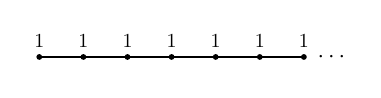
\begin{tikzpicture}[baseline=-.5ex,x=.56cm,y=.56cm]
  \foreach \x in {0,...,6}{
    \fill (\x,0) circle (1.05pt);
    \node[above=1pt,scale=.72] at (\x,0) {$1$};
  }
  \draw (0,0)--(6,0);
  \node[right=2pt,scale=.85] at (6,0) {$\cdots$};
\end{tikzpicture}
\\

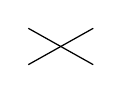
\begin{tikzpicture}[baseline=-.5ex,x=.55cm,y=.55cm]
  \draw[line width=.45pt] (-.75,-.42)--(.75,.42);
  \draw[line width=.45pt] (-.75,.42)--(.75,-.42);
\end{tikzpicture}
& $xy=0$ & $1$ &
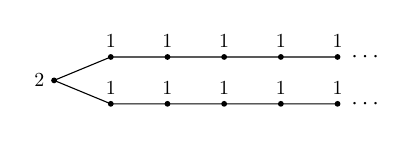
\begin{tikzpicture}[baseline=-.5ex,x=.72cm,y=.62cm]
  \fill (0,0) circle (1.05pt);
  \node[left=1pt,scale=.72] at (0,0) {$2$};
  \foreach \x in {1,...,5}{
    \fill (\x,.48) circle (1.05pt);
    \fill (\x,-.48) circle (1.05pt);
    \node[above=1pt,scale=.72] at (\x,.48) {$1$};
    \node[above=1pt,scale=.72] at (\x,-.48) {$1$};
  }
  \draw (0,0)--(1,.48)--(5,.48);
  \draw (0,0)--(1,-.48)--(5,-.48);
  \node[right=2pt,scale=.85] at (5,.48) {$\cdots$};
  \node[right=2pt,scale=.85] at (5,-.48) {$\cdots$};
\end{tikzpicture}
\\

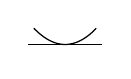
\begin{tikzpicture}[baseline=-.5ex,x=.55cm,y=.55cm]
  \draw[line width=.45pt] (-.85,0)--(.85,0);
  \draw[line width=.45pt,domain=-.72:.72,samples=40]
    plot (\x,{.72*\x*\x});
\end{tikzpicture}
& $y(y-x^2)=0$ & $2$ &
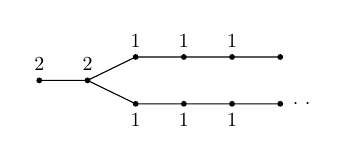
\begin{tikzpicture}[baseline=-.5ex,x=.68cm,y=.62cm]
  \fill (0,0) circle (1.05pt);
  \fill (.9,0) circle (1.05pt);
  \node[above=1pt,scale=.72] at (0,0) {$2$};
  \node[above=1pt,scale=.72] at (.9,0) {$2$};
  \foreach \x/\lab in {1.8/1,2.7/1,3.6/1,4.5/0}{
    \fill (\x,.48) circle (1.05pt);
    \fill (\x,-.48) circle (1.05pt);
    \ifnum\lab=1
      \node[above=1pt,scale=.72] at (\x,.48) {$1$};
      \node[below=1pt,scale=.72] at (\x,-.48) {$1$};
    \fi
  }
  \draw (0,0)--(.9,0)--(1.8,.48)--(4.5,.48);
  \draw (.9,0)--(1.8,-.48)--(4.5,-.48);
  \node[right=2pt,scale=.72] at (4.5,-.48) {$\cdot\ \cdot$};
\end{tikzpicture}
\\

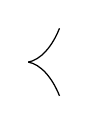
\begin{tikzpicture}[baseline=-.5ex,x=.55cm,y=.55cm]
  \draw[line width=.45pt]
    (0,0) .. controls (.28,.05) and (.55,.35) .. (.72,.78);
  \draw[line width=.45pt]
    (0,0) .. controls (.28,-.05) and (.55,-.35) .. (.72,-.78);
\end{tikzpicture}
& $y^2=x^3$ & $1$ &
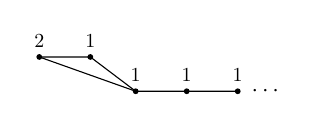
\begin{tikzpicture}[baseline=-.5ex,x=.72cm,y=.65cm]
  \coordinate (A) at (0,.42);
  \coordinate (B) at (.9,.42);
  \coordinate (C) at (1.7,-.25);
  \coordinate (D) at (2.6,-.25);
  \coordinate (E) at (3.5,-.25);
  \foreach \p in {A,B,C,D,E}{\fill (\p) circle (1.05pt);}
  \node[above=1pt,scale=.72] at (A) {$2$};
  \foreach \p in {B,C,D,E}{\node[above=1pt,scale=.72] at (\p) {$1$};}
  \draw (A)--(B)--(C)--(D)--(E);
  \draw (A)--(C);
  \node[right=2pt,scale=.85] at (E) {$\cdots$};
\end{tikzpicture}
\end{tabular}
\end{center}


Si $n>2$, el invariante $\delta$ ya no está determinado por este diagrama. Por
ejemplo, la unión de tres rectas concurrentes coplanarias (respectivamente, no
coplanarias) tiene invariante $\delta=3$ (respectivamente, $\delta=2$), aunque
el diagrama de Enriques sea el mismo. No sé si este fenómeno se produce también
para las curvas unirrama.

He aquí dos ejemplos de diagramas en el caso $n=3$ que no pueden aparecer para
curvas planas (cf.~2.5). Damos, por orden, las ecuaciones de la curva, las
ecuaciones de la transformada estricta después de la explosión del origen, unas
ecuaciones paramétricas de la curva, el invariante $\delta$ y el diagrama de
Enriques.

\pageoriginale

\begin{equation}\tag{2.25.1}
\left\{
\begin{gathered}
  \left\{\begin{aligned}y^2&=xz^4,\\ z^3&=x^2,
  \end{aligned}\right.\qquad
  \left\{\begin{aligned}(y/z)^2&=(x/z)^3,\\ z&=(x/z)^2,
  \end{aligned}\right.\\[3pt]
  \left\{\begin{aligned}x&=u^6,\\y&=u^7,\\z&=u^4,
  \end{aligned}\right.\qquad \delta=5
\end{gathered}
\right.
\end{equation}

\begin{center}
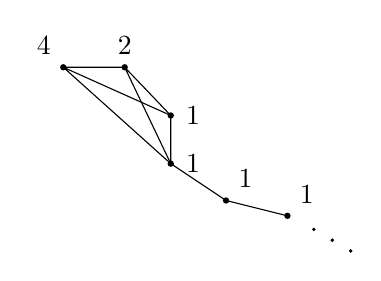
\begin{tikzpicture}[x=.78cm,y=.72cm]
  \coordinate (v1) at (0,0);
  \coordinate (v2) at (1,0);
  \coordinate (v3) at (1.75,-.85);
  \coordinate (v4) at (1.75,-1.70);
  \coordinate (v5) at (2.65,-2.35);
  \coordinate (v6) at (3.65,-2.62);
  \foreach \p in {v1,v2,v3,v4,v5,v6}{\fill (\p) circle (1.15pt);}
  \node[above left=1pt] at (v1) {$4$};
  \node[above=1pt] at (v2) {$2$};
  \node[right=2pt] at (v3) {$1$};
  \node[right=2pt] at (v4) {$1$};
  \node[above right=1pt] at (v5) {$1$};
  \node[above right=1pt] at (v6) {$1$};
  \draw (v1)--(v2) (v1)--(v3) (v1)--(v4);
  \draw (v2)--(v3) (v2)--(v4) (v3)--(v4);
  \draw (v4)--(v5)--(v6);
  \fill (4.08,-2.86) circle (.7pt);
  \fill (4.38,-3.05) circle (.7pt);
  \fill (4.68,-3.24) circle (.7pt);
\end{tikzpicture}
\end{center}

\begin{equation}\tag{2.25.2}
\left\{
\begin{gathered}
  \left\{\begin{aligned}y^2z&=x^3,\\ z^3&=y^2,
  \end{aligned}\right.\qquad
  \left\{\begin{aligned}(y/z)^2&=(x/z)^3,\\ z&=(y/z)^2,
  \end{aligned}\right.\\[3pt]
  \left\{\begin{aligned}x&=u^8,\\y&=u^9,\\z&=u^6,
  \end{aligned}\right.\qquad \delta=10
\end{gathered}
\right.
\end{equation}

\begin{center}
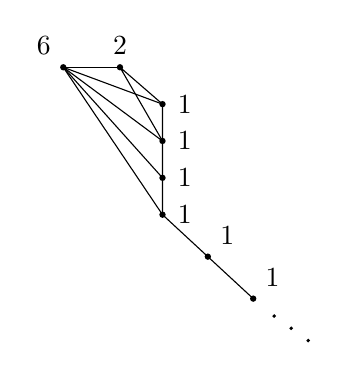
\begin{tikzpicture}[x=.72cm,y=.65cm]
  \coordinate (w1) at (0,0);
  \coordinate (w2) at (1,0);
  \coordinate (w3) at (1.75,-.72);
  \coordinate (w4) at (1.75,-1.44);
  \coordinate (w5) at (1.75,-2.16);
  \coordinate (w6) at (1.75,-2.88);
  \coordinate (w7) at (2.55,-3.70);
  \coordinate (w8) at (3.35,-4.52);
  \foreach \p in {w1,w2,w3,w4,w5,w6,w7,w8}{\fill (\p) circle (1.15pt);}
  \node[above left=1pt] at (w1) {$6$};
  \node[above=1pt] at (w2) {$2$};
  \foreach \p in {w3,w4,w5,w6}{\node[right=2pt] at (\p) {$1$};}
  \node[above right=1pt] at (w7) {$1$};
  \node[above right=1pt] at (w8) {$1$};
  \draw (w1)--(w2);
  \foreach \p in {w3,w4,w5,w6}{\draw (w1)--(\p);}
  \draw (w2)--(w3) (w2)--(w4);
  \draw (w3)--(w4)--(w5)--(w6)--(w7)--(w8);
  \fill (3.72,-4.86) circle (.7pt);
  \fill (4.02,-5.10) circle (.7pt);
  \fill (4.32,-5.34) circle (.7pt);
\end{tikzpicture}
\end{center}


\subsection*{2.26}
El Teorema 2.27 que sigue fue enunciado como conjetura falsa en la primera
versión de esta exposición (difundida por el IHÉS). Debe mucho a conversaciones con
D.~S. Rim e incluye algunos resultados suyos (D.~S. Rim, ``Torsion
Differentials and Deformations'', Teorema 2.7(i)).

\pageoriginale

Sea $C$ una curva proyectiva reducida sobre un cuerpo algebraicamente cerrado
$k$, y sea $s\in C(k)$. Escribiremos:
\begin{description}
\item[$A_s$] el anillo local de $C$ en $s$ (o su completado, lo que no cambia
nada en lo que sigue);
\item[$\widetilde A_s$] la normalización de $A_s$;
\item[$\delta(s)$] el número $\dim_k(\widetilde A_s/A_s)$;
\item[$m_0(s)$] la dimensión del esquema formal versal $T$ de deformaciones de
$\operatorname{Spec}(A_s)$.
\end{description}

Para una componente irreducible $E$ de $T$, pongamos asimismo
$m_0^E(s)=\dim(E)$.

El módulo $\widetilde\tau$ de las derivaciones de $\widetilde A_s$ y el módulo
$\tau$ de las derivaciones de $A_s$ son libres de torsión. Si
$\sisi{A}{A_s}$ es íntegro, se sumergen en el módulo de derivaciones del cuerpo
de fracciones de $A_s$; en general, se sumergen en el módulo de derivaciones del
anillo total de cocientes de $A_s$ (un producto de cuerpos). Además, mediante
estas inmersiones, $\tau$ y $\widetilde\tau$ son conmensurables: tanto
$\tau/(\tau\cap\widetilde\tau)$ como
$\widetilde\tau/(\tau\cap\widetilde\tau)$ son de dimensión finita sobre $k$.
Pongamos
\begin{equation*}
m_1(s)=[\widetilde\tau:\tau]
\mathrel{\mathop=\limits_{\mathrm{def}}}
\dim_k\frac{\widetilde\tau}{\tau\cap\widetilde\tau}
-\dim_k\frac{\tau}{\tau\cap\widetilde\tau}.
\end{equation*}

\medskip
\noindent\underline{Teorema 2.27.}
\underline{Sea $E$ una componente irreducible del esquema formal versal $T$ de
deformaciones de $A_s$. Si la deformación de $A_s$ sobre el punto genérico $e$
de $E$ es lisa ---es decir, si la imagen del subesquema formal de no lisitud
(definido por un ideal jacobiano: VI 5), que es finito sobre $T$, no contiene a
$e$---, entonces}
\begin{equation*}
3\delta(s)=m_0^E(s)+m_1(s).
\end{equation*}

\pageoriginale

La validez de 2.27 solo depende del completado de $A_s$. Reemplazando $(C,s)$
por un par $(C',s)$ formalmente isomorfo a él en $s$, podemos suponer que se
cumplen las condiciones siguientes:

\medskip
\noindent (a) $s$ es el único punto singular de $C$;

\noindent (b) $C$ no tiene automorfismos infinitesimales.

La condición (b) asegura que el funtor de deformaciones de $C$ es
prorepresentable. Es incluso efectivamente prorepresentable, pues no hay
obstrucción para levantar un haz invertible amplio prescrito sobre $C$. Sea
$f:X_0\longrightarrow T_0$ la deformación universal de $C$, y sea $t_0$ el
punto cerrado de $T_0$, de modo que
$C\overset\sim\longrightarrow X_{0t_0}$.

\medskip
\noindent\underline{Lema 2.28.}
\underline{Existen un esquema $T_1$ de tipo finito sobre $k$, un punto
$t_1\in T_1(k)$ y un morfismo propio y plano $f:X_1\longrightarrow T_1$, cuya
fibra en $t_1$ es $C$, tales que, para todo $u\in T_1(k)$, el completado de
$T_1$ en $u$ es un esquema formal de módulos para la fibra $X_{1u}$.}

He aquí una demostración directa de este corolario de resultados generales de
Artin. Sea $\mathcal L$ un haz invertible muy amplio sobre $C$ tal que
$H^1(C,\mathcal L)=0$, y pongamos
$\mathbb P=\mathbb P(H^{\sisi{o}{0}}(C,\mathcal L))$. Tenemos una inmersión
$v:C\hookrightarrow\mathbb P$. Sea $T_2$ el esquema de Hilbert que parametriza
las subvariedades de $\mathbb P$ con el mismo polinomio de Hilbert que
$v(C)\subset\mathbb P$, y sea $t_2\in T_2$ el punto correspondiente a $v(C)$.
El completado $\widehat T_2$ de $T_2$ en $t_2$ es liso sobre
$\sisi{S_o}{T_o}$. El fibrado tangente vertical de
$\widehat T_2/T_o$ está inducido por el subfibrado $L$ del fibrado tangente de
$T_2$ que es la imagen de
$\operatorname{Lie}(\underline{\operatorname{Aut}}(\mathbb P))$ mediante la
acción de $\underline{\operatorname{Aut}}(\mathbb P)$ sobre $T_2$.

En un entorno de $t_2$, sean $f_1,\ldots,f_n$, con
$n=\dim\underline{\operatorname{Aut}}(\mathbb P)$, unas ecuaciones que definen
un subesquema $T'_1$ de $T_2$ que pasa por $t_2$ y cuyo completado en $t_2$ es
étale sobre $T_0$. Tomemos como $T_1$ un entorno de
$\sisi{t}{t_2}$ en $T'_1$ sobre el cual el fibrado tangente sea transversal a
$L$.

\pageoriginale

\subsection*{2.29}
El morfismo de funtores
\begin{equation*}
(\text{deformaciones de }C)\longrightarrow
(\text{deformaciones de }A_s)
\end{equation*}
corresponde a un morfismo $p:T_0\longrightarrow T$. Por VI 2.10, $p$ es liso.
Sea $t$ el punto cerrado de $T$. El espacio tangente de Zariski a $p^{-1}(t)$
en $t_0$ clasifica las deformaciones localmente triviales de $C$ sobre
$k[\varepsilon]$, donde $\varepsilon^2=0$. Poniendo $E_0=p^{-1}(E)$, obtenemos
\begin{equation}\tag{2.29.1}
\dim(E_0)=\dim(E)+\dim H^1(C,T^1_{C/k}).
\end{equation}

Como $X_0/T_0$ es plano, todas sus fibras tienen el mismo género aritmético
$p$, donde $1-p=\chi(\underline O)$. Por hipótesis, la fibra en el punto
genérico de $E_0$ es lisa. Puesto que el esquema formal de módulos de una curva
propia lisa es liso de dimensión $3p-3$, el Lema 2.28 da
\begin{equation}\tag{2.29.2}
\dim(\sisi{E}{E_0})=3p-3.
\end{equation}

Sea $\widetilde C$ la normalización de $C$, de género aritmético
$\widetilde p=p-\delta(s)$. Se tiene
\begin{equation}\tag{2.29.3}
\begin{aligned}
\dim H^1(C,T^1_{C/k})
&=-\chi(C,T^1_{C/k})\\
&=-\chi(\widetilde C,T^1_{\widetilde C/k})+m_1(s)\\
&=\sisi{-}{}[3(p-\delta(s))-3]+m_1(s).
\end{aligned}
\end{equation}

Las fórmulas (2.29.1), (2.29.2) y (2.29.3) demuestran 2.27.

\medskip
\noindent\underline{Conjetura 2.30.}
\underline{Toda curva propia reducida admite una deformación lisa.}

Esta conjetura implica, por 2.27 y 2.28, que el esquema formal versal de
deformaciones de $A_s$ es siempre equidimensional, de dimensión
$3\delta(s)-m_1(s)$.

\pageoriginale

\subsection*{2.31}
Sea $C$ una curva propia reducida sobre $k$, de género aritmético $p$.
Escribiremos:
\begin{description}
\item[$M_0$] la dimensión del esquema formal versal $T$ de deformaciones de
$C$;
\item[$M_1$] la dimensión del álgebra de Lie de
$\underline{\operatorname{Aut}}(C)$.
\end{description}

Para una componente irreducible $E$ de $T$, designemos por $M_0^E$ la dimensión
de $E$. El análogo global de 2.27 es el siguiente.

\medskip
\noindent\underline{Proposición 2.32.}
\underline{Si la deformación de $C$ sobre el punto genérico de $E$ es lisa,
entonces}
\begin{equation*}
3p-3=M_0^E-M_1.
\end{equation*}

Sea $X\subset C(k)$ un conjunto finito de puntos lisos de $C$ tal que todo campo
de vectores sobre $C$ que se anule en cada punto $x\in X$ sea nulo. El funtor
de deformaciones de $(C,X)$ es prorepresentable y satisface una variante de
2.28. El esquema formal de módulos de $(C,X)$ es liso sobre $T$, de dimensión
relativa $\#X-M_1$, y el análogo de 2.28 da
\begin{equation*}
\sisi{M_0}{M_0^E}+(\#X-M_1)=3p-3+\#X,
\end{equation*}
lo que demuestra 2.32.

Supongamos ahora que $k$ es de \underline{característica cero}. Entonces
$M_1=\dim\underline{\operatorname{Aut}}(C)$. He aquí una interpretación análoga
de $m_1(s)$.

\pageoriginale

\medskip
\noindent\underline{Lema 2.33.}
\underline{Si $k$ es de característica cero, toda derivación de $A_s$ se
extiende a una derivación de $\widetilde A_s$.}

Si $D$ es una derivación de $A_s$, entonces
\begin{equation*}
\exp(Dt)=\sisi{\sum}{\sum_{n\geq0}}\frac{D^nt^n}{n!}
\end{equation*}
es un automorfismo del completado en $(s,0)$ de $A_s\otimes_k k[t]$. Por
transporte de estructura, este automorfismo actúa sobre la normalización
$(\widetilde A_s\otimes_k k[t])^{\wedge}$ de este anillo. Reduciendo módulo
$t^2$, se obtiene un automorfismo $1+Dt$ de
$\widetilde A_s^{\wedge}\otimes_k k[t]/(t^2)$, y $D$ se extiende así a una
derivación de $\widetilde A_s^{\wedge}$. Puesto que se extiende también al
cuerpo de fracciones de $A_s$ (al anillo total de cocientes cuando $A_s$ no es
íntegro), se extiende a $\widetilde A_s$.

Supongamos que $s$ es singular. Un argumento análogo muestra entonces que el
campo de vectores sobre $\operatorname{Spec}(\widetilde A_s)$ definido por $D$
se anula en todo punto situado sobre $s$.

Sea $c$ un ideal de $\widetilde A_s$ contenido en el conductor de
$\widetilde A_s/A_s$. Pongamos
\begin{equation*}
\widetilde G_c=\underline{\operatorname{Aut}}(\widetilde A_s/c),
\end{equation*}
y sea $G_c$ el subgrupo de $\widetilde G_c$ que estabiliza la subálgebra
$A_s/c$. Si $d\subset c$, entonces $\widetilde G_d$ estabiliza $c/d$ y se
aplica sobre $\widetilde G_c$. Obsérvese que
$g\in\widetilde G_c$ está determinado por $g(t)$ para un uniformizante $t$, y
que $g(t)$ puede ser un uniformizante cualquiera. Por consiguiente, el espacio
homogéneo apuntado $\widetilde G_c/G_c$ es independiente de $c$; lo designamos
por $\widetilde G/G$.

Sea $\widetilde\tau_0$ el $\widetilde A_s$-módulo de los campos de vectores
sobre $\operatorname{Spec}(\widetilde A_s)$ que se anulan en los puntos
situados sobre $s$. Cuando $s$ es singular, se tiene
\begin{equation*}
\dim_k(\widetilde\tau/\widetilde\tau_0)
=\text{el número de ramas},
\end{equation*}
y
\begin{equation*}
\widetilde\tau_0/\tau\overset\sim\longrightarrow
\text{el espacio tangente en el origen de }\widetilde G/G.
\end{equation*}

\pageoriginale

\medskip
\noindent\underline{Proposición 2.34.}
\underline{En característica cero, cuando $s$ es singular, el entero $m_1(s)$
es la suma del número de ramas y de la dimensión de $\widetilde G/G$.}

\bigskip
\begin{center}
\underline{\textsc{Bibliografía}}
\end{center}

\begin{description}
\item[{[1]}] P. Defrise, \textit{Étude locale des correspondances rationnelles
entre surfaces algébriques}, tesis de agregación, Bruselas, 1949.

\item[{[2]}] P. Deligne y D. Mumford, ``The irreducibility of the space of
curves of a given genus'', \textit{Publ. Math. IHES} \underline{36} (1969),
75--110.

\item[{[3]}] Enriques--Chisini, \textit{Lezioni sulla teoria geometrica delle
equazioni \sisi{et}{e} delle funzioni algebriche}, Zanichelli, Bolonia, 1924.

\item[{[4]}] R. Hartshorne, \textit{Residues and Duality},
\sisi{Lectures}{Lecture} Notes in Math. \underline{20},
Springer, 1966.

\item[{[5]}] S. Lichtenbaum, ``Curves over discrete valuation rings'',
\textit{Amer. J. Math.} \sisi{15}{90}, núm.~2 (abril de 1968), 380--405.

\item[{[6]}] I. Manin, ``Rational surfaces over perfect fields'',
\textit{Publ. Math. IHES}, núm.~30, 55--114.

\item[{[7]}] D. Mumford, ``The topology of normal singularities of an algebraic
\sisi{surfaces}{surface} and a criterion for simplicity'',
\textit{Publ. Math. IHES}, núm.~9, 5--22.

\item[{[8]}] A. Néron, \textit{Modèles minimaux des variétés abéliennes sur
les corps locaux et globaux}, Publ. Math., núm.~21.

\pageoriginale

\item[{[9]}] M. Raynaud, ``Spécialisation du foncteur de Picard. Critères
numériques de représentabilité'', \textit{C. R. Acad. Sci. Paris} 264
(junio de 1967), 1001--1004.

\item[{[10]}] Saint-Donat, \textit{Sur un théorème de G. Castelnuovo et
F. Enriques}, tesis de tercer ciclo, Lyon.

\item[{[11]}] O. Zariski, ``On polynomial ideals defined by infinitely near
base points\sisi{}{,}'', \textit{Amer. J. Math.} 60 (1938), 151.

\item[{[12]}] D. G. Northcott, ``On the genus formula for plane curves'',
\textit{J. London Math. Soc.} 30 (1955), 376--382.

\item[{[13]}] D. G. Northcott, ``Abstract dilatations and infinitely near
points'', \textit{Proc. Cambridge Philos. Soc.} 52 (1956), 178--197.

\item[] La noción de ``punto infinitamente próximo'' se estudia en el apéndice
de Lipman al Capítulo II de la obra siguiente.

\item[{[14]}] O. Zariski, \textit{Algebraic Surfaces}, Ergebnisse
\underline{61}, \sisi{Springer Verlag}{Springer-Verlag}.
\end{description}

